% Source-backed observations; no reconstruction or prediction results.
% Natural subfigure layout: images share one baseline and one height, no panel
% frames. Panel width follows each image's own aspect ratio, so the four
% thumbnails are not forced into identical boxes.
\begingroup
\linespread{1}\selectfont
\begin{tikzpicture}[x=1cm,y=1cm,text=black,
  font=\songti\fontsize{9.5pt}{12pt}\selectfont,
  every node/.style={align=center,inner sep=0pt,outer sep=0pt}]
  \path[use as bounding box] (0,0.30) rectangle (16,3.95);

  \def\imgh{2.05cm}
  % Common baseline at y = 1.55; centres follow from the column widths above.
  \node[anchor=south] at (1.95,1.55)
    {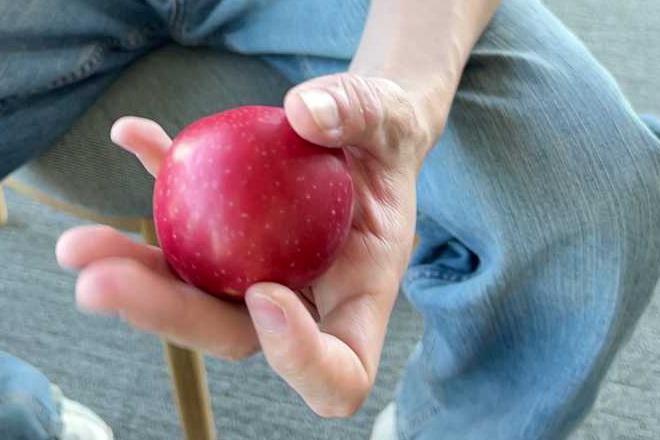
\includegraphics[height=\imgh]{figures/generated/evaluation/dycheck_a.png}};
  \node[anchor=south] at (5.95,1.55)
    {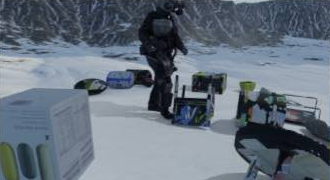
\includegraphics[height=\imgh]{figures/generated/evaluation/pointodyssey_snow.png}};
  \node[anchor=south] at (9.85,1.55)
    {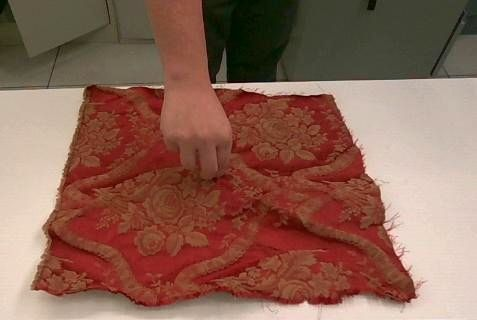
\includegraphics[height=\imgh]{figures/generated/evaluation/phystwin_a.png}};
  \node[anchor=south] at (13.85,1.55)
    {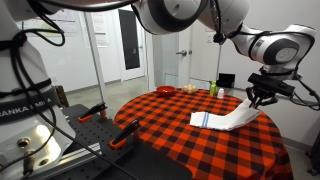
\includegraphics[height=\imgh]{figures/generated/evaluation/droid_view1.png}};

  % Panel letters are numbered by the caption package, not typed into the TikZ
  % code, so each one can be cross-referenced with \subref.
  \foreach \xx/\paneltitle/\lab in {%
      1.95/{DyCheck iPhone}/{datasets-dycheck},%
      5.95/{PointOdyssey}/{datasets-pointodyssey},%
      9.85/{PhysTwin}/{datasets-phystwin},%
      13.85/{DROID}/{datasets-droid}}{%
    \node[text width=3.6cm,align=center] at (\xx,1.24)
      {{\captionsetup[subfigure]{font=figsubsongti,skip=0pt}
      \subcaption{\paneltitle}\label{subfig:\lab}}};
  }
  \foreach \xx/\note in {1.95/{真实采集、单目视频},5.95/{合成场景、轨迹标注},
                         9.85/{可控变形、交互序列},13.85/{真实机器人操作}}{
    \node[font=\fontsize{8.8pt}{11pt}\selectfont,text=black!70] at (\xx,0.92) {\note};
  }
\end{tikzpicture}
\endgroup
